% !TeX program = xelatex
% !TeX encoding = UTF-8 Unicode
% !BIB program = biblatex

\documentclass[english]{sencir}

\title{SENCIR \LaTeX ~model (2024)} %Title is made uppercase automatically

\addbibresource{references.bib}

\setid{XX-00} %The ID was sent by e-mail

\setemail{corresponding.author@institution.com} %Just put the corresponding author e-mail

\addauthor{First Author}{1}
\addauthor{Second Author}{2}
\addauthor{Third Author}{1}

\addinstitution{1}{First institution, address} %Author of same institution should have the same identification
\addinstitution{2}{Second institution, address}

\addkeyword{keyword 1}%Use 3 to 5 keywords
\addkeyword{keyword 2}
\addkeyword{keyword 3}

\preamble{}

\begin{document} %Maximum of 8 pages
    \maketitle{}
    
    % Abstract
    \begin{abstract} %Maximum of 400 words.
        The abstract should be no more than 400 words.
    \end{abstract}
    
    \section{intrOdUCTION} %Section is made uppercase automatically
    
        The work can be written in Portuguese, English, or Spanish and may contain a %When you break 1 line, LaTeX understand you keep in the same paragraph.
        maximum of 6 to 8 pages, including references.

        Paragraph. %If you braeak 2 or more lines, LaTeX understand you want to change the paragraph.
        
        \subsection{SubSection}
            Important note: this \LaTeX document uses the \texttt{xelatex} compiler instead
            of \texttt{pdflatex}. If you use \texttt{latexmk}, it is already configured
            corretly. If you are using an editor, be it online or offline, make sure to
            configure it to use \texttt{xelatex}. The reason is that \texttt{xelatex} is
            simply better, handling, fonts, accents and UTF-8 characteres natively, without
            the need to include \texttt{inputenc}. The generated PDF is also better quality,
            specially for accents.

            \subsubsection{SubSubSection}
                Send the complete work in PDF format by July 31, 2024, at the latest, through
                the platform indicated on the website www.sencir.nuclear.ufmg.br.
    
    \section{METHODOLOGY}
    
        Describe here the methodology and/or the procedures and materials used to carry
        out the work \citep{bibExemple}. 
    
        As said by \citet{bibExemple} did so, so and so, as in
        \Cref{fig:label-fig1}.
    
        \begin{figure}[h]
            %You can use the H (H in uppercase) option inside [] to make the picture "HERE", but it's not recommended.
            %Let LaTeX figure out the best position to figures and tables.
            %Imagens and table should be after you first ref it, don't matter how much far from the first ref.
            \centering
            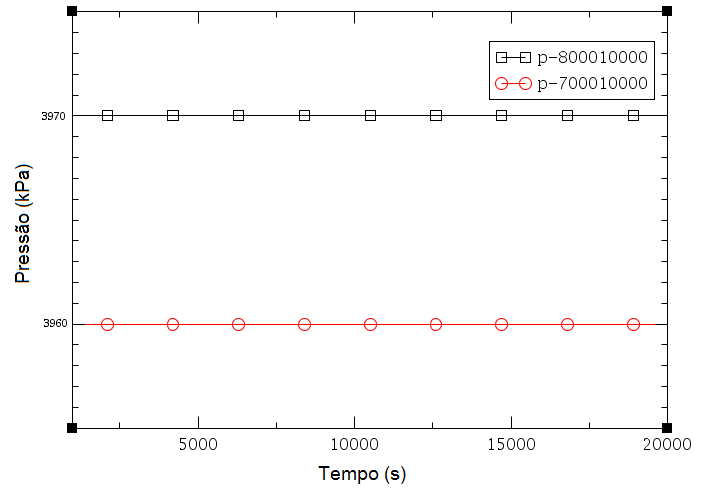
\includegraphics[height=6cm]{Picture1.png}
            \caption{Example fig}
            \label{fig:label-fig1}
        \end{figure}
    
    \section{RESULTS}
    
        In this section, describe the main results and their analyses, as can see in \Cref{tab:label-tab1}.
    
        \begin{table}[h]
            \begin{tabular}{l@{\hspace{0.6cm}}l}
                  \toprule
                   {\textbf{Item}}   & {\textbf{Value}} \\
                  \midrule
                   {Item1}           & {Value1}         \\
                   {Item2}           & {Value2}         \\
                   {Item3}           & {Value3}
                  \vspace{0.2cm}                        \\
                   {Item4}           & {Value4}         \\
                   {Item5}           & {Value5}         \\
                   {Item6}           & {Value6}         \\
                   {Item7}           & {Value7}         \\
                   {Item8}           & {Value8}         \\
                   \bottomrule
            \end{tabular}
            \caption{Example tab}%
            \label{tab:label-tab1}
        \end{table}
    
    \section{CONCLUSION}
    
        Main conclusions. 
        
        Important: the work must have a maximum of 8 pages, including references.
    
    \section*{ACKNOWLEDGEMENTS}
    
        Thank the funding bodies, collaborators, institutions, etc., if any.
    
    \printbibliography
    
\end{document}
